%% ----------------------------------------------------------------
%% Implementation.tex
%% ---------------------------------------------------------------- 

\chapter{System Implementation} \label{Chapter:System Implementation}

This chapter will give detailed information about the implementation of this system. It will start with the introduction of the implementation technologies and tools for this system. Afterwards, this chapter will explain how the main components of this system are implemented to conform to the requirement specifications.


\section{Technologies and Tools
}
Appropriate implementation technologies and tools are the keys to the success of a software system, while poor choices may cause difficulties, delays or even failure of a software system. Regarding the system analysis and design, the following technologies and tools are chosen to develop this system. 



\subsection{Programming Language}

JavaScript is chosen as the main programming language for developing this system. There are several reasons for this choice. Firstly, AngularJS is a JavaScript-based front-end framework, so it is natural to choose JavaScript as the programming language. Secondly, many third-party libraries, like D3.js, for data visualisation are written in JavaScript. Last but not the least, JavaScript, which is the most popular programming language in the world \cite{ARC}, has a big community and a variety of tutorials, which makes it easy to develop and maintain this system. 


\subsection{Development Framework}

In order to build this system rapidly and efficiently, AngularJS, a commonly-used front-end framework is chosen to develop this system. More narrowly, the framework of this system is MVVM pattern, as explained in chapter 5. This pattern allows the developers to write better organized, and therefore more maintainable system, so it a good choice for developing this system.

\subsection{User Interface}

Apart from AngularJS, some basic building technologies of the front-end development are used for the web interface design. HTML5 is used for structuring and presenting content on the web interface, and CSS3 is used for describing the presentation of a document written in HTML5.
 
\subsection{Data Visualisation}

Regarding with the objectives of this project, some data visualisation technologies are chosen to visualize open data. Highcharts.js is a charting library written in JavaScript, offering an easy way of adding interactive charts to the website web application. It is used to visualize weather data from OpenWeatherMap API and provide international students with data visualisation about the weather information of cities. 

Although highcharts.js can provide developers with a rapid way of adding charts in the web pages, it only has limited choices of charts. Hence, D3.js is also used in this system to visualize crime data from Police API. It is a JavaScript library that allows developers to build the data visualisation framework they want. Besides, the requirements analysis in chapter 4 suggests that the location of universities and the environment of cities are crucial factors influencing international students’ decision-making process. So, Google Maps JavaScript API is applied in this system to visualize the geographical information and the infrastructure of cities.


\subsection{Development Tools}

There are two main development tools used for this system. One tool is Github, a version control tool for managing this system and keeping track of the changes in code, and another one is Atom, an integrated development environment (IDE) for developing the web application of this project.

\subsection{Deployment Platform}

In order to allow the users access to this system at anytime and anyplace, this system is published online, and the website for this system is \href{http://univguide.netlify.com/#/}{http://univguide.netlify.com/\#/}. Specifically, the front-end of this system is deployed with Netlify and the back-end (Node.js proxy) is deployed with Heroku.


\section{System Components Implementation}

Based on the system analysis and design, some components are built to implement this system. This section will explain the main components of this system with some screenshots and necessarily codes presented. 


\subsection{Search Bar
}	
As shown in the use case diagram, most components of this system rely on the search results, so the search bar is the most important functionality of this system. The first step for the users is to search universities and courses while using this system. 

\begin{figure}[H]
  \centering
  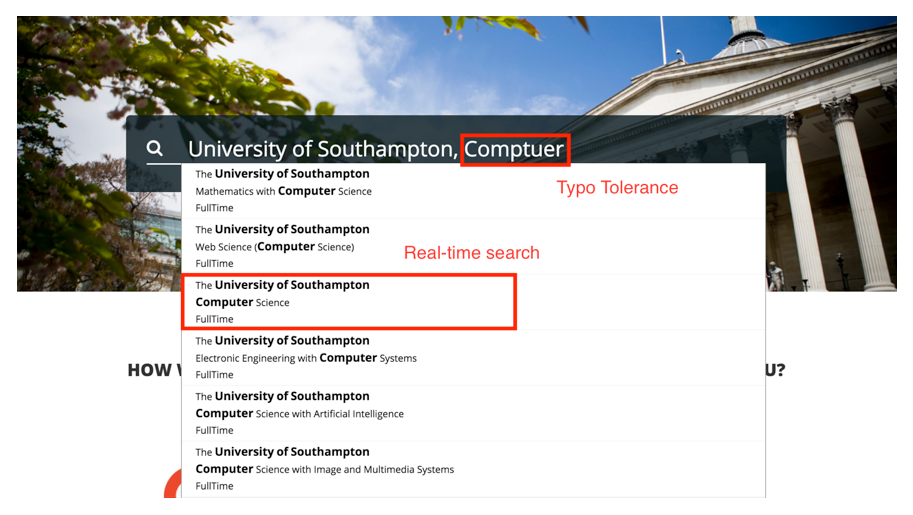
\includegraphics[width=15cm]{./img/Picture16}
  \caption{Search Bar}
  \label{Figure:figex}
\end{figure}

\begin{figure}[H]
  \centering
  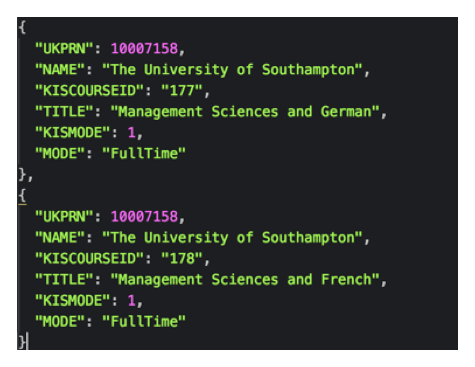
\includegraphics[width=6cm]{./img/Picture17}
  \caption{University Name, Course Title and Corresponding Identifiers
}
  \label{Figure:figex}
\end{figure}

In order to improve the user experience, the search bar is implemented using Algolia \cite{Alogolia} for real-time search and typo tolerance (see Figure 6.1). Another reason for using Algolia is that \$http.get() requests sent to Unistats API can only take the identifiers of universities and courses as parameters, so it is necessary to covert the users’ searching inputs (university names and course titles) to corresponding identifiers (UKPRN and KISCOURSEID) before sending those requests to Unistats API. The JSON file (see Figure 6.2) that contains university names and course titles as well as their corresponding identifiers is stored in Algolia. 








When the users enter university names and course titles, the suggestions will show up and the matched results will be highlighted. Once the suggestions are selected, the search bar will convert the inputs to their corresponding identifiers and send \$http.get() requests containing these identifiers to Unistats API. 

\subsection{University \& Course}

The University\&Course part provides some basic information about universities and courses, such as tuition fee and living expense, to help the users gain quick insights into them. Figure 6.3 shows part of information displayed in University\&Course part. 

\begin{figure}[H]
  \centering
  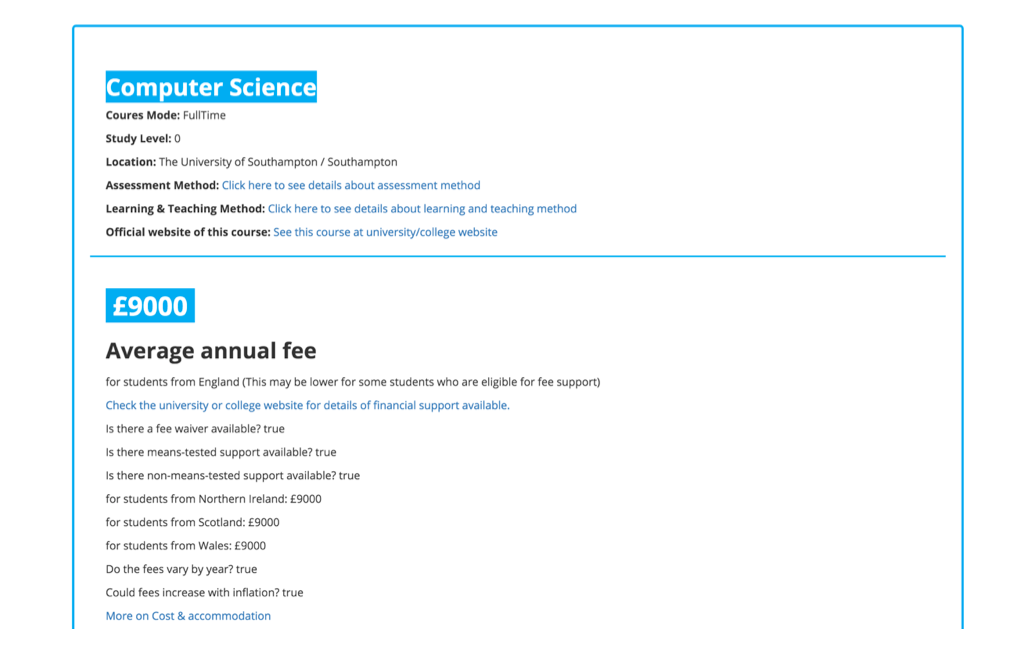
\includegraphics[width=15cm]{./img/Picture18}
  \caption{Part Information in University \& Course Part}
  \label{Figure:figex}
\end{figure}


\begin{figure}[H]
  \centering
  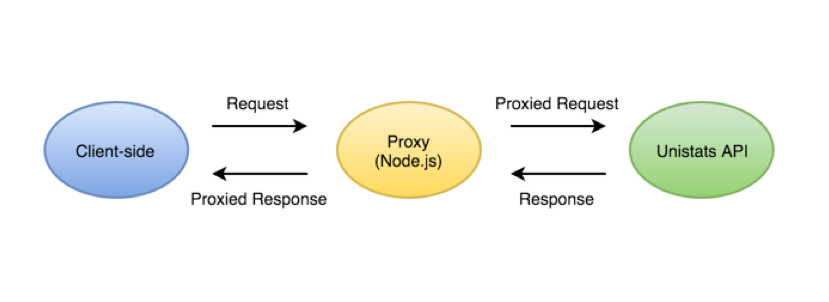
\includegraphics[width=12cm]{./img/Picture19}
  \caption{Back-end Proxy
}
  \label{Figure:figex}
\end{figure}

As discussed above, four \$http.get() requests will be sent to Unistats API to get information about the selected universities and courses, but the problem is that \$http.get() requests sent from the client side is not allowed by Unistats API. To solve this problem, Node.js is used in this system to allow these requests through a server side proxy and have the server side proxy return the data back to the client side (see Figure 6.4).

\begin{figure}[H]
  \centering
  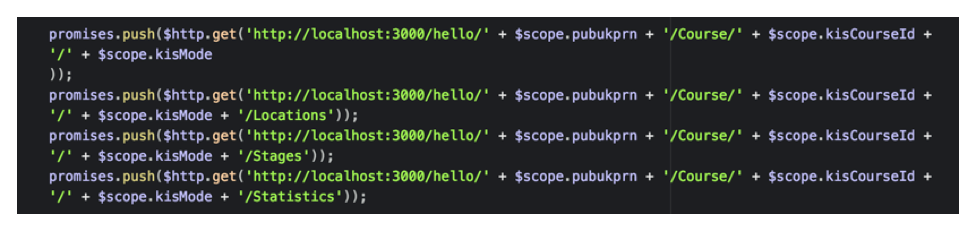
\includegraphics[width=15cm]{./img/Picture20}
  \caption{Front-end Requests}
  \label{Figure:figex}
\end{figure}


As shown in Figure 6.5, an endpoint (/hello) is set up to grab these four requests to the server side. The client side will send those parameters to the port of the server side after receiving the search results from the search bar. Afterwards, the server side proxy will send the proxied requests (see Figure 6.6) to Unistats API and return responses to the client side. Finally, the front-end will display the proxied responses on the webpage. 

\begin{figure}[H]
  \centering
  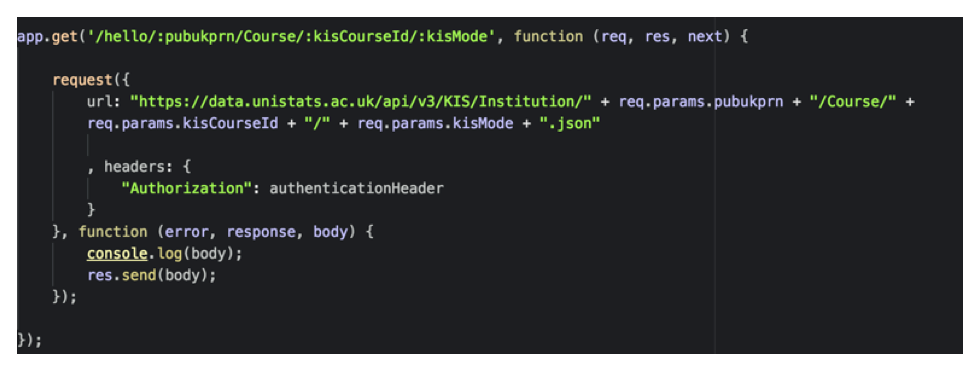
\includegraphics[width=15cm]{./img/Picture21}
  \caption{One of Back-end Proxied Requests
}
  \label{Figure:figex}
\end{figure}



\subsection{Ranking Table}

The ranking table (see Figure 6.7) of this system provides the users with the ranking and the score variation of all ranking criteria of universities in the UK. Moreover, the users are allowed to interact with the ranking table. For example, the users can reorder the ranking table according to different ranking criteria. 

\begin{figure}[H]
  \centering
  \includegraphics[width=15cm]{./img/Picture22}
  \caption{Ranking Table Part}
  \label{Figure:figex}
\end{figure}


\subsection{Course Location}

As mentioned in section 5.3.3, the browser will send requests containing the geolocation data (latitude and longitude) about cities to other open APIs used in this system. Therefore, the Course Location part (see Figure 6.8) can provide information about the locations of cities when the users search for universities. Assuming the user wants to search computer science in University of Southampton, the browser will send requests containing the identifiers of University of Southampton and computer science to Unistats API. Then, Unistats API will return data about computer science in University of Southampton with the geolocation data about Southampton to the browser. After receiving the geolocation data, the browser will send it to Google Map Matrix API, which is used to display the location of Southampton on the map. Also, Google Map Matrix API is used to calculate the distances and driving time between Southampton and several metropolises, like London and Manchester, which can help the users to gain an insight into the location of Southampton at ease.

\begin{figure}[H]
  \centering
  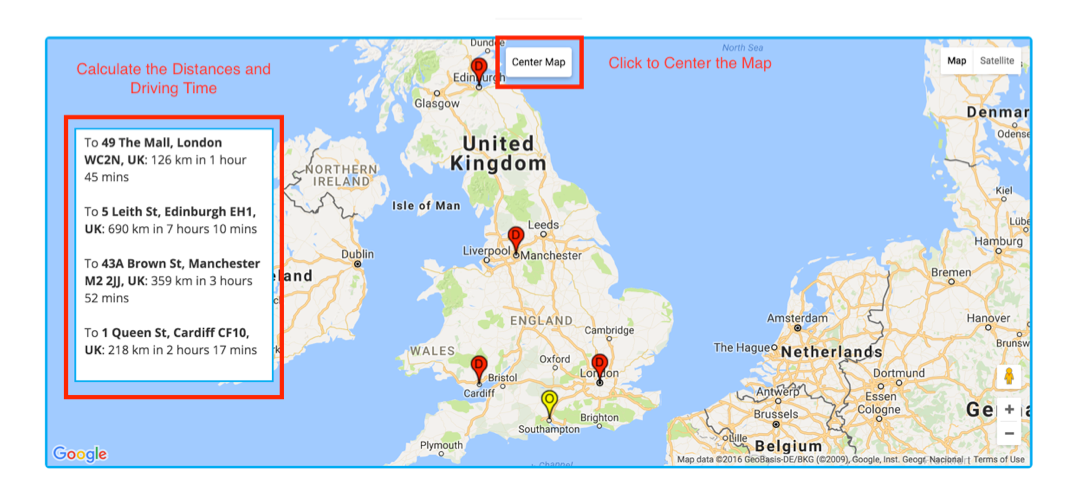
\includegraphics[width=15cm]{./img/Picture23}
  \caption{Course Location Part}
  \label{Figure:figex}
\end{figure}


\subsection{Weather}




According to the geolocation data from Unistats API, the weather part can get data about the weather in different cities from OpenWeatherMap API (see Figure 6.9) and visualize it using highchart.js (see Figure 6.10).

\begin{figure}[H]
  \centering
  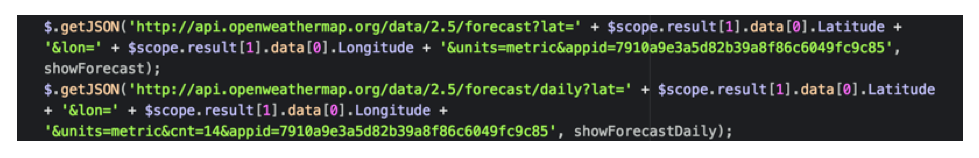
\includegraphics[width=15cm]{./img/Picture24}
  \caption{Requests Sent to OpenWeatherMap API
}
  \label{Figure:figex}
\end{figure}

\begin{figure}[H]
  \centering
  \includegraphics[width=15cm]{./img/Picture25}
  \caption{Weather Part
}
  \label{Figure:figex}
\end{figure}

Figure 6.10 presents the weather forecast in Southampton. Specifically, these two charts display the variations of temperature and precipitation in next hours and next 14 days in Southampton respectively. Moreover, the users are allowed to interact with the charts. For instance, the users can hover over the charts and see the tooltips. 




\subsection{Criminality}

The criminality part provides a map that visualizes the crime data of different cities, and this can provide a great understanding of the safety of cities. As shown in Figure 6.11, the crime data of Southampton in May 2016 is visualized in the circles of different colours and sizes, and the tooltips of the circles give the users more details about the crimes in a certain location. On the other hand, the panel on the left gives an overview of the crime data. The pie chart shows the colours and the percentages of different types of crimes and the drop-down box allows the users to select the crime data in different months.

\begin{figure}[H]
  \centering
  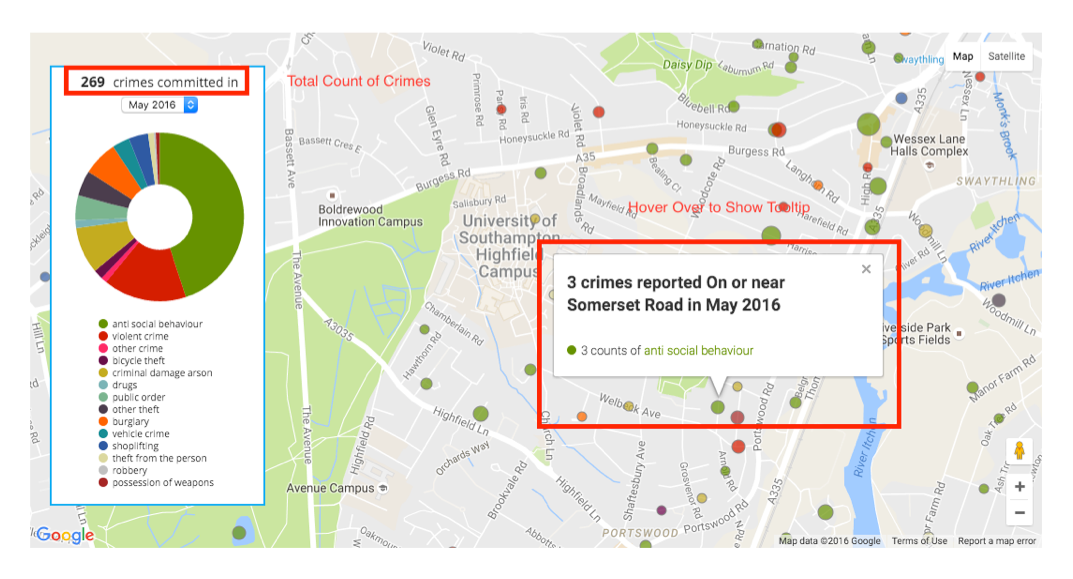
\includegraphics[width=15cm]{./img/Picture26}
  \caption{Criminality Part
}
  \label{Figure:figex}
\end{figure}


\subsection{Infrastructure}

The infrastructure part displays a map that allows the users to know the locations of different kinds of infrastructure in cities. As shown in Figure 6.11, if the users want to know the locations of train stations and movie theatres in Southampton, the browser will send corresponding requests to Google Map Places API and display the responses on the map with different markers. If there are no selected kinds of infrastructure, like embassy, in cities, the browser will pop up a window (see Figure 6.12) to remind the users.


\begin{figure}[H]
  \centering
  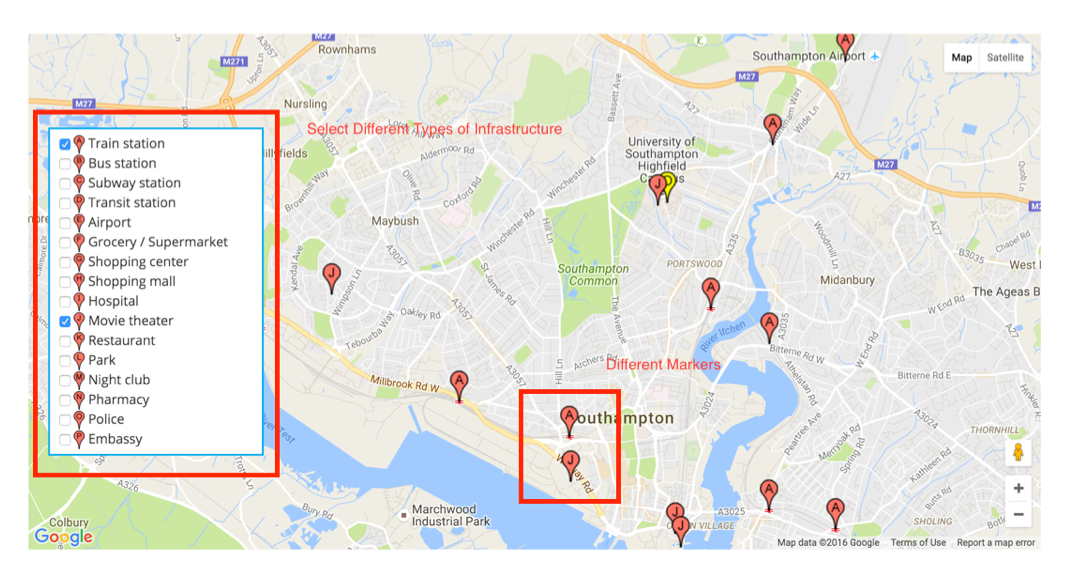
\includegraphics[width=15cm]{./img/Picture27}
  \caption{Infrastructure Part}
  \label{Figure:figex}
\end{figure}

\begin{figure}[H]
  \centering
  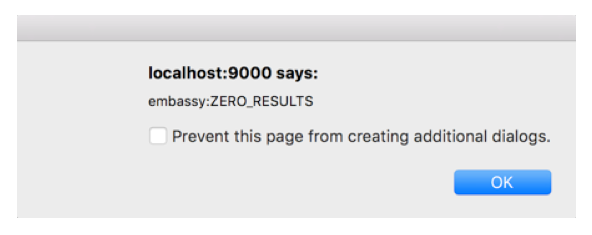
\includegraphics[width=8cm]{./img/Picture28}
  \caption{Zero Results}
  \label{Figure:figex}
\end{figure}



\section{Summary}


This chapter focuses on the implementation of this system. At first, this chapter briefly introduces the technologies and tools used for implementing this system. Then, it explains how the main components of this system are implementation with several screenshots and part of codes provided.

